\documentclass[border=5pt]{standalone}
\usepackage{tikz}
\usepackage{amsmath}
\usetikzlibrary{positioning, arrows.meta, calc, fit, backgrounds, shapes.geometric}

% --- Color Scheme (Blue-Gray) ---
\definecolor{bgPrimary}{HTML}{DAE8FC}
\definecolor{bgSecondary}{HTML}{E8EEF7}
\definecolor{bgAccent}{HTML}{B3CDE3}
\definecolor{bgInput}{HTML}{F0F4F8}
\definecolor{borderPrimary}{HTML}{6C8EBF}
\definecolor{borderAccent}{HTML}{3A6EA5}
\definecolor{arrowColor}{HTML}{4A6A8A}
\definecolor{textMain}{HTML}{2C3E50}
\definecolor{textLight}{HTML}{7F8C8D}
\definecolor{bgHighlight}{HTML}{FFF3CD}

% --- Styles ---
\tikzset{
  module/.style={draw=borderPrimary, fill=bgPrimary, rounded corners=4pt,
    minimum width=2.8cm, minimum height=1.2cm,
    font=\sffamily\small, text=textMain, line width=0.6pt, align=center},
  novelmodule/.style={draw=borderAccent, fill=bgAccent, rounded corners=4pt,
    minimum width=2.8cm, minimum height=1.2cm,
    font=\sffamily\small\bfseries, text=textMain, line width=1.0pt, align=center},
  iobox/.style={draw=borderPrimary, fill=bgInput, rounded corners=3pt,
    minimum width=2cm, minimum height=1cm,
    font=\sffamily\small, text=textMain, line width=0.5pt, align=center},
  stdarrow/.style={-{Stealth[length=5pt, width=4pt]}, line width=0.6pt, color=arrowColor},
  groupbox/.style={draw=borderPrimary, fill=bgSecondary, fill opacity=0.3,
    rounded corners=6pt, inner sep=8pt, line width=0.5pt, dashed},
  devbox/.style={draw=borderPrimary, fill=bgInput, rounded corners=3pt,
    minimum width=1.6cm, minimum height=0.7cm,
    font=\sffamily\scriptsize, text=textMain, line width=0.5pt, align=center},
  agentbox/.style={draw=borderPrimary, fill=bgPrimary, rounded corners=3pt,
    minimum width=1.8cm, minimum height=0.7cm,
    font=\sffamily\scriptsize, text=textMain, line width=0.5pt, align=center},
  widebox/.style={draw=borderPrimary, fill=bgPrimary, rounded corners=4pt,
    minimum width=8.0cm, minimum height=1.0cm,
    font=\sffamily\small, text=textMain, line width=0.6pt, align=center},
  widenovel/.style={draw=borderAccent, fill=bgAccent, rounded corners=4pt,
    minimum width=8.0cm, minimum height=1.0cm,
    font=\sffamily\small\bfseries, text=textMain, line width=1.0pt, align=center},
}

\begin{document}
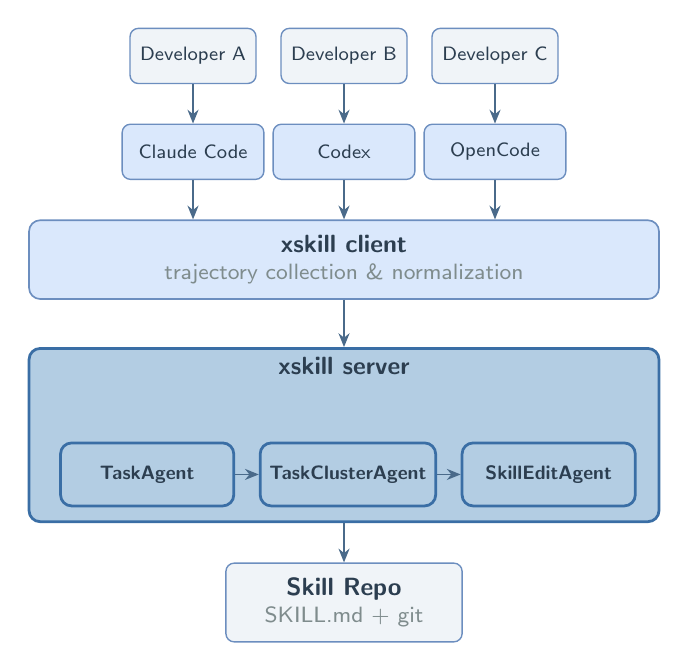
\begin{tikzpicture}

  % === Row 1: Developers ===
  \node[devbox] (devA) {Developer A};
  \node[devbox, right=0.3cm of devA] (devB) {Developer B};
  \node[devbox, right=0.3cm of devB] (devC) {Developer C};

  % === Row 2: Coding Agents (below developers) ===
  \node[agentbox, below=0.5cm of devA] (cc) {Claude Code};
  \node[agentbox, below=0.5cm of devB] (codex) {Codex};
  \node[agentbox, below=0.5cm of devC] (oc) {OpenCode};

  % Arrows: dev -> agent
  \draw[stdarrow] (devA) -- (cc);
  \draw[stdarrow] (devB) -- (codex);
  \draw[stdarrow] (devC) -- (oc);

  % === Row 3: xskill client ===
  \coordinate (agentMid) at ($(cc.south)!0.5!(oc.south)$);
  \node[widebox, below=0.5cm of agentMid, anchor=north] (client) {%
    \textbf{xskill client}\\[-1pt]
    {\footnotesize\color{textLight} trajectory collection \& normalization}};

  % Arrows: agents -> client
  \draw[stdarrow] (cc.south) -- (cc.south |- client.north);
  \draw[stdarrow] (codex.south) -- (codex.south |- client.north);
  \draw[stdarrow] (oc.south) -- (oc.south |- client.north);

  % === Row 4: xskill server (group containing 3 agents) ===
  \node[widenovel, below=0.6cm of client, minimum height=2.2cm] (server) {};
  \node[font=\sffamily\small\bfseries, text=textMain, anchor=north] at (server.north) {xskill server};

  % Three pipeline agents inside server
  \node[novelmodule, minimum width=2.2cm, minimum height=0.8cm,
    font=\sffamily\scriptsize\bfseries] (ta) at ([yshift=-0.5cm, xshift=-2.5cm]server.center) {TaskAgent};
  \node[novelmodule, minimum width=2.2cm, minimum height=0.8cm,
    font=\sffamily\scriptsize\bfseries, right=0.3cm of ta] (tca) {TaskClusterAgent};
  \node[novelmodule, minimum width=2.2cm, minimum height=0.8cm,
    font=\sffamily\scriptsize\bfseries, right=0.3cm of tca] (sea) {SkillEditAgent};

  % Arrows inside server
  \draw[stdarrow] (ta) -- (tca);
  \draw[stdarrow] (tca) -- (sea);

  % Arrow: client -> server
  \draw[stdarrow] (client) -- (server);

  % === Row 5: Skill Repo ===
  \node[iobox, below=0.5cm of server, minimum width=3cm] (repo) {%
    \textbf{Skill Repo}\\[-1pt]
    {\footnotesize\color{textLight} SKILL.md + git}};

  % Arrow: server -> repo
  \draw[stdarrow] (server) -- (repo);

\end{tikzpicture}
\end{document}
